\documentclass{article}
\usepackage{xcolor}
\usepackage{listings}
\usepackage{booktabs}
\usepackage{amsmath}
\usepackage{tcolorbox}
\usepackage{array}
\usepackage{graphicx}
\usepackage{multirow}
\usepackage{fancyvrb}
\usepackage{tabularx}
\usepackage{url}
\usepackage{tikz}
\pagestyle{myheadings}

\begin{document}
\section{What is this document?}
This document contains theory and related practice problems to help students prepare for Midterm Exam 1 of the CS-4400 Spring 2025 course, taught by Prof. Dr. John Regehr at the University of Utah. It covers topics that students have asked about most frequently. Additional information is provided through links to Compiler Explorer, which include useful comments, assembly code, and even visualized stack diagrams in the comments. Please refer to them as you read.

For errors and additional information, please refer to the Acknowledgement section (\S\ref{sec:ack}).
\clearpage
\section{Register info}
\renewcommand{\arraystretch}{1.5}
\setlength{\tabcolsep}{8pt}

\begin{table}[h]
    \centering
    \begin{tabular}{|c|c|c|c|l|}
        \hline
        \multicolumn{4}{|c|}{\textbf{Bit Ranges}} & \multirow{2}{*}{\textbf{Description}} \\
        \cline{1-4}
        63 & 31 & 15 & 7 &  \\
        \hline
        \%rax  & \%eax  & \%ax  & \%al  & Return value \\
        \%rbx  & \%ebx  & \%bx  & \%bl  & Callee saved \\
        \%rcx  & \%ecx  & \%cx  & \%cl  & 4th argument \\
        \%rdx  & \%edx  & \%dx  & \%dl  & 3rd argument \\
        \%rsi  & \%esi  & \%si  & \%sil & 2nd argument \\
        \%rdi  & \%edi  & \%di  & \%dil & 1st argument \\
        \%rbp  & \%ebp  & \%bp  & \%bpl & Callee saved \\
        \%rsp  & \%esp  & \%sp  & \%spl & Stack pointer \\
        \%r8   & \%r8d  & \%r8w  & \%r8b  & 5th argument \\
        \%r9   & \%r9d  & \%r9w  & \%r9b  & 6th argument \\
        \%r10  & \%r10d & \%r10w & \%r10b & Caller saved \\
        \%r11  & \%r11d & \%r11w & \%r11b & Caller saved \\
        \%r12  & \%r12d & \%r12w & \%r12b & Callee saved \\
        \%r13  & \%r13d & \%r13w & \%r13b & Callee saved \\
        \%r14  & \%r14d & \%r14w & \%r14b & Callee saved \\
        \%r15  & \%r15d & \%r15w & \%r15b & Callee saved \\
        \hline
    \end{tabular}
    \caption{Breakdown of x86-64 General Purpose Registers. Remember, the register itself is 64 bits wide (0–63). Certain portions of it have specific names. We do not have separate registers for 64-bit \%rax, 32-bit \%eax, etc. Instead, there is a single 64-bit \%rax register, and its lower 32 bits are referred to as \%eax.}
    \label{tab:x86_64_registers}
\end{table}
\clearpage
\subsection{Calling Conventions - How parameters are passed to a function}
\label{sec: how-args-passed}
The arguments are passed to a function using the registers:
\begin{verbatim}
    %rdi, %rsi, %rdx, %rcx, %r8, %r9
\end{verbatim}
or by using other parts of these registers, such as \texttt{\%edi, \%esi, ...} or \texttt{\%dil, \%sil, ...}, depending on the size of the value. If there are more than six arguments, the additional arguments are stored on the stack. \\
See an example here: \url{https://godbolt.org/z/Yesv1Mo9d} \\

\subsection{Calling Conventions - Callee and Caller saved registers}
\label{sec: calle-caller-regs}
%
The ABI defines callee-saved registers as: \\
\\
%
\textit{A function can use one of these registers if it saves it first. The function must restore the register’s original value before exiting.} \\
\\
%
This means that the value of the register must be restored; in other words, it must have the same value before and after a function call. \\
%
\noindent For example:
\begin{verbatim}
mov $0, %rbp    # %rbp has value 0
call fun_uses_rbp()
cmpq $0, %rbp   # %rbp still has the same value 0.
\end{verbatim}
%
Since \texttt{\%rbp} is callee-saved, the function \texttt{fun\_uses\_rbp()} can use \texttt{\%rbp}, but it must restore the previous value before exiting. That is why \texttt{\%rbp} has the same value (0) before and after the call to \texttt{fun\_uses\_rbp()}. \\
%
On the other hand, caller-saved (or \textbf{not} callee-saved) registers may have different values before and after a function call. The callee function is not responsible for saving or restoring their values; instead, the caller function must save their values if they are needed after the function call. \\
%
\noindent For example:
\begin{verbatim}
mov $0, %rax    # %rax has value 0
call fun_uses_rax()
cmpq $0, %rax   # %rax can have a different value 
\end{verbatim}
%
Since \texttt{\%rax} is not callee-saved, the function \texttt{fun\_uses\_rax()} is not responsible for restoring its previous value. As a result, \texttt{\%rax} may hold a different value after the function call.
%
\subsection{Calling Conventions - More information}
Register \texttt{\%rax} holds the return value. \\
\noindent For example, for the following C code:
\begin{verbatim}
long multiply(long a, long b) {
    long return_value = a * b;
    return return_value;
}
\end{verbatim}
\noindent the following assembly code has been generated:
\begin{verbatim}
multiply:
        movq    %rdi, %rax
        imulq   %rsi, %rax
        ret
\end{verbatim}

As you can see, \texttt{\%rax} is used as the register that is returned in the end. \\

See the code here: \url{https://godbolt.org/z/EjsPf5r7o} \\
\\

Register \texttt{\%rsp} is used as the stack pointer, a pointer to the topmost element in the stack.
\clearpage
\section{Simple moves}
\subsection{Move with different sizes}
\begin{table}[h]
    \centering
    \small
    \renewcommand{\arraystretch}{1.2}
    \begin{tabular}{l l c c}
        \toprule
        \textbf{C declaration} & \textbf{Intel data type} & \textbf{Assembly-code suffix} & \textbf{Size (bytes)} \\
        \midrule
        char/unsigned char     & Byte             & b  & 1 \\
        short/unsigned short    & Word             & w  & 2 \\
        int/unsigned int      & Double word      & l  & 4 \\
        long/unsigned long     & Quad word        & q  & 8 \\
        char* (or any pointer)  & Quad word        & q  & 8 \\
        float    & Single precision & s  & 4 \\
        double   & Double precision & l  & 8 \\
        \bottomrule
    \end{tabular}
    \caption{Sizes of C data types in x86-64. With a 64-bit machine, pointers are 8 bytes long.}
    \label{tab:c_data_types}
\end{table}


\noindent\textbf{Related Problem 1} (Updated from Practice Problem 3.2)

\vspace{5pt}

For each of the following lines of assembly language, determine the appropriate instruction suffix based on the operands. (For example, \texttt{mov} can be rewritten as \texttt{movb}, \texttt{movw}, \texttt{movl}, or \texttt{movq}.) \\
%
\textbf{Hint:} Choose the suffixes that are compatible with the smaller-sized register. You can extract one byte from an 8-byte register, but you cannot extract 8 bytes from a 1-byte register.
%

\vspace{10pt}

\begin{lstlisting}[basicstyle=\ttfamily, frame=none]
mov__   %eax, (%rsp)        
mov__   (%rax), %dx         
mov__   $0xFF, %bl          
mov__   (%rsp,%rdx,4), %d1  
mov__   (%rdx), %rax        
mov__   %dx, (%rax)        
\end{lstlisting} 
%
\noindent\textbf{Related Problem 2} (Updated from Practice Problem 3.3)

\vspace{5pt}

Each of the following lines of code generates an error message when we invoke the assembler. Explain what is wrong with each line and write the corrected version.

\vspace{10pt}

\begin{lstlisting}[basicstyle=\ttfamily, frame=none]
movb  $0xF, (%ebx)    | Correct version: 
movl  %rax, (%rsp)    | Correct version:
movw  (%rax), 4(%rsp) | Correct version:
movb  %al, %sl        | Correct version:
movq  %rax, $0x123    | Correct version:
movl  %eax, %rdx      | Correct version:
movb  %si, 8(%rbp)    | Correct version:
\end{lstlisting}

\clearpage % Forces a new page

\subsection{Move with Extensions}

\begin{table}[t] % Ensures the table stays at the top of the page
    \centering
    \small
    \renewcommand{\arraystretch}{1.1}
    \begin{tabular}{l l l}
        \toprule
        \textbf{Instruction} & \textbf{Effect} & \textbf{Description} \\
        \midrule
        \multicolumn{3}{c}{\textbf{Sign-Extending Instructions}} \\
        \midrule
        \texttt{movs} $S, R$  & $R \leftarrow \text{SignExtend}(S)$ & Move with sign extension \\
        \texttt{movsbw} &  & Move sign-extended byte to word \\
        \texttt{movsbl} &  & Move sign-extended byte to double word \\
        \texttt{movswl} &  & Move sign-extended word to double word \\
        \texttt{movsbq} &  & Move sign-extended byte to quad word \\
        \texttt{movswq} &  & Move sign-extended word to quad word \\
        \texttt{movslq} &  & Move sign-extended double word to quad word \\
        \texttt{cltq}   & \%rax $\leftarrow$ SignExtend(\%eax) & Sign-extend \%eax to \%rax \\
        \midrule
        \midrule % Thicker line for section change
        \multicolumn{3}{c}{\textbf{Zero-Extending Instructions}} \\
        \midrule
        \texttt{movz} $S, R$  & $R \leftarrow \text{ZeroExtend}(S)$ & Move with zero extension \\
        \texttt{movzbw} &  & Move zero-extended byte to word \\
        \texttt{movzbl} &  & Move zero-extended byte to double word \\
        \texttt{movzwl} &  & Move zero-extended word to double word \\
        \texttt{movzbq} &  & Move zero-extended byte to quad word \\
        \texttt{movzwq} &  & Move zero-extended word to quad word \\
        \texttt{movzlq (not exist)} &  & \textbf{!!! Why do we not have this?} \\
        \bottomrule
    \end{tabular}
    \caption{Move with extensions. As you notice, we do not have \texttt{movzlq} because it would be unnecessary based on the following conventions.}
\end{table}

\noindent\textbf{Register Updates Based on Data Movement Instructions}

\vspace{5pt}

As there are two conventions for data movement, the remaining bytes in the register are affected differently:
\begin{itemize}
    \item Instructions generating \textbf{1- or 2-byte} quantities leave the remaining bytes unchanged.
    \item Instructions generating \textbf{4-byte} quantities set the upper 4 bytes of the register to zero.
\end{itemize}

\vspace{10pt}

\begin{lstlisting}[basicstyle=\ttfamily, frame=none, numbers=left, numberstyle=\color{blue}]
movabsq $0x0011223344556677, %rax    %rax = 0011223344556677
movb    $-1, %al                     %rax = 00112233445566FF
movw    $-1, %ax                     %rax = 001122334455FFFF
movl    $-1, %eax                    %rax = 00000000FFFFFFFF
movq    $-1, %rax                    %rax = FFFFFFFFFFFFFFFF
\end{lstlisting}

That is why \texttt{movl \$-1, \%eax} moves the value to \%eax and automatically \texttt{zero-extends} (zeros out the upper 4 bytes) due to the conventions mentioned above. You may also see \texttt{movl \%eax, \%eax}, which is a simple trick to zero out the upper bytes.

\textbf{FWIW:} Do not worry about \texttt{movabsq \$0x0011223344556677, \%rax}; it is simply used to move very large numbers. When a 64-bit number can be represented as a 32-bit value, the compiler uses \texttt{mov}. If it cannot, then it uses \texttt{movabsq}. 

\texttt{movabsq} can have a register as its destination, but it cannot write directly to memory. See an example here:
\url{https://godbolt.org/z/bsvjGsf3G} \\
\\
Most of the time you will see \texttt{xorl \%eax, \%eax} that is used to zero out the \texttt{\%rax}. Based on the Table~\ref{truth-table} xoring the same value with itself will result in zero. Since zeroing \texttt{\%eax} also zeros out the upper 4 bytes, compiler chooses \texttt{xorl \%eax, \%eax} which is a cheaper than \texttt{movq \$0, \%rax}\\

\noindent\textbf{Related Problem 3} (Updated from Practice Problem 3.5)

\vspace{5pt}

You are given the following information. A function with the prototype:

\begin{lstlisting}[basicstyle=\ttfamily, frame=none]
void decode(long *xp, long *yp, long *zp);
\end{lstlisting}

is compiled into assembly code, yielding the following:

\begin{lstlisting}[basicstyle=\ttfamily, frame=none]
decode:
    movq    (%rdi), %r8
    movq    (%rsi), %rcx
    movq    (%rdx), %rax
    movq    %r8, (%rsi)
    movq    %rcx, (%rdx)
    movq    %rax, (%rdi)
    ret
\end{lstlisting}

\vspace{5pt}

Parameters \texttt{xp}, \texttt{yp}, and \texttt{zp} are stored in registers \_\_\_\_, \_\_\_\_, and \_\_\_\_, respectively (Remember calling conventions from\S\ref{sec: how-args-passed}.)

\vspace{5pt}

Write C code for \texttt{decode} that will have an effect equivalent to the assembly code shown.\\
\begin{lstlisting}[basicstyle=\ttfamily, frame=none]
// Complete the function below
void decode(long *xp, long *yp, long *zp) {







}
\end{lstlisting}
\textit{Answer: }\url{https://godbolt.org/z/9G4696P6j} \\
\clearpage
\noindent\textbf{Related Problem 4} (Updated from Practice Problem 3.4)

\begin{lstlisting}
void cast(TYPE_1 *sp, TYPE_2 *dp) {
    *dp = (TYPE_2) *sp;
}
\end{lstlisting}

You are given this function that casts a source value (\texttt{*sp}) and writes it to a destination (\texttt{*dp}). Write the instructions necessary to perform the same operation with different \texttt{TYPE\_1} and \texttt{TYPE\_2}. An example is provided for you.

\textbf{Remember:}
\begin{itemize}
    \item \textbf{You cannot move from memory to memory.}
    \item When performing a cast that involves both a \textbf{size change} and a \textbf{change of signedness} in C, the operation should change the size first.
\end{itemize}

\vspace{10pt}

\begin{table}[h]
    \centering
    \small
    \renewcommand{\arraystretch}{1.4} % Adjusts row height for two lines
    \begin{tabular}{l l p{5cm}} % p{5cm} allows two-line content
        \toprule
        \textbf{TYPE\_1} & \textbf{TYPE\_2} & \textbf{Instruction} \\
        \midrule
        long & long & \texttt{movq (\%rdi), \%rax} \newline \texttt{movq \%rax, (\%rsi)} \\
        char & int & \underline{\hspace{5cm}} \newline \underline{\hspace{5cm}} \\
        char & unsigned & \underline{\hspace{5cm}} \newline \underline{\hspace{5cm}} \\
        unsigned char & long & \underline{\hspace{5cm}} \newline \underline{\hspace{5cm}} \\
        int & char & \underline{\hspace{5cm}} \newline \underline{\hspace{5cm}} \\
        unsigned & unsigned char & \underline{\hspace{5cm}} \newline \underline{\hspace{5cm}} \\
        char & short & \underline{\hspace{5cm}} \newline \underline{\hspace{5cm}} \\
        \bottomrule
    \end{tabular}
\end{table}
\\
\textit{Answer: }\url{https://godbolt.org/z/ePox4Y7sv}
\clearpage
\section{Arithmetic and Logical Operations}
\subsection{Basic operations}
\begin{table}[h]
    \centering
    \small
    \renewcommand{\arraystretch}{1.2}
    \begin{tabular}{l l l}
        \toprule
        \textbf{Instruction} & \textbf{Effect} & \textbf{Description} \\
        \midrule
        \texttt{leaq} $S, D$  & $D \leftarrow \&S$ & Load effective address \\
        \midrule
        \texttt{INC} $D$  & $D \leftarrow D+1$ & Increment \\
        \texttt{DEC} $D$  & $D \leftarrow D-1$ & Decrement \\
        \texttt{NEG} $D$  & $D \leftarrow -D$ & Negate \\
        \texttt{NOT} $D$  & $D \leftarrow \sim D$ & Complement \\
        \midrule
        \texttt{ADD} $S, D$  & $D \leftarrow D + S$ & Add \\
        \texttt{SUB} $S, D$  & $D \leftarrow D - S$ & Subtract \\
        \texttt{IMUL} $S, D$  & $D \leftarrow D * S$ & Multiply \\
        \texttt{XOR} $S, D$  & $D \leftarrow D  \^\ S$ & Exclusive-or \\
        \texttt{OR} $S, D$  & $D \leftarrow D | S$ & Or \\
        \texttt{AND} $S, D$  & $D \leftarrow D \& S$ & And \\
        \midrule
        \texttt{SAL} $k, D$  & $D \leftarrow D << k$ & Left shift \\
        \texttt{SHL} $k, D$  & $D \leftarrow D << k$ & Left shift (same as \texttt{SAL}) \\
        \texttt{SAR} $k, D$  & $D \leftarrow D >>_A k$ & Arithmetic right shift \\
        \texttt{SHR} $k, D$  & $D \leftarrow D >>_L k$ & Logical right shift \\
        \bottomrule
    \end{tabular}
    \caption{Common arithmetic and logical instructions in x86-64. The \texttt{leaq} (Load Effective Address) instruction is commonly used to perform simple arithmetic. The remaining ones are more standard unary or binary operations. We use the notation \texttt{>>} for right shifts, with signed values using \textit{arithmetic right shift} (`SAR`) and unsigned values using \textit{logical right shift} (`SHR`). Logical right shift puts ZEROS to the beginning while Atithmetic right shift puts the SIGN BIT (0 or 1) to the beginning. Additionally, all of them sets the condition flags except \texttt{lea}
}
\label{basic-arith}
\end{table}

As you notice, an operation is performed, and the result is written to the destination. Remember that all of them take \texttt{D} as the first argument:

\begin{verbatim}
add S, D   # D = D + S  (D comes first)
sub S, D   # D = D - S  (D comes first)
\end{verbatim}

\noindent
\textbf{Related Problem 5} (Updated from Practice Problem 3.10)

\begin{lstlisting}
short calc(short a, short b, short c) {

    short d = ______;
    short e = ______;
    short f = ______;
    short g = ______;
    return g;
    
}
\end{lstlisting}

The generated assembly code implementing these expressions is as follows:

\begin{lstlisting}
calc:
    movl    %esi, %eax
    orl     %esi, %edi
    sarw    $11, %di
    notl    %edi
    subl    %edi, %eax
    ret
\end{lstlisting}

\noindent
\textbf{Based on this assembly code, fill in the missing portions of the C code above.} \\
\\
\textit{Answer: }\url{https://godbolt.org/z/aq9h3G8h8}
\subsection{LEA (Load effective address)}
First, let us remember the equation that is used to access certain parts of memory:
\noindent 
\\
\begin{tcolorbox}[colframe=black, colback=white, boxrule=1pt]
    \begin{equation*}
        \text{Memory} \quad \textit{Imm}(r_b, r_i, s) = M[\textit{Imm} + R[r_b] + R[r_i] \cdot s]
    \end{equation*}
    \caption{Operands can denote immediate (constant) values, register values, or values from memory. The scaling factor \( s \) must be either 1, 2, 4, or 8.}
    \label{equation_mem}
\end{tcolorbox}
%
\noindent
%
In Related Problem 6, we will apply our equation to determine the memory address and then \textit{dereference} that address to access the value stored at it.
%
The \texttt{LEA} instruction works in a similar way, but it \textbf{DOES NOT DEREFERENCE} the memory.
For example, imagine that register \%rax holds the value \texttt{0x10}. Additionally, the memory address \texttt{0x14} contains the value \texttt{0x20}. When we execute the instruction:
%
\[
\texttt{movq 4(\%rax), \%rsi}
\]
%
First, the \texttt{mov} instruction takes the value in \%rax, which is \texttt{0x10}. Then, based on the equation above, it adds \texttt{4} to this value: \texttt{0x10 + 4 = 0x14}. After that, it dereferences the memory address \texttt{0x14}, which holds the value \texttt{0x20}, and moves this value into the \%rsi register. \\
%
If we use the \texttt{LEA} instruction instead:
%
\[
\texttt{leaq 4(\%rax), \%rsi}
\]
%
The instruction computes \texttt{0x10 + 4 = 0x14} and moves this computed address directly into the \%rsi register without dereferencing the memory at \texttt{0x14}. As the name implies, \texttt{LEA} (Load Effective Address) loads the address, not the value stored at that address. \\
\\
%
\noindent\textbf{Related Problem 6} (Updated from Practice Problem 3.1) \\
Assume the following values are stored at the indicated memory addresses and registers:

\begin{table}[h!]
    \centering
    \small
    \renewcommand{\arraystretch}{1.2}
    \begin{tabular}{ll ll}
        \toprule
        \textbf{Address} & \textbf{Value} & \textbf{Register} & \textbf{Value} \\
        \midrule
        0x100 & 0xFF  & \%rax & 0x100 \\
        0x104 & 0xAB  & \%rcx & 0x1 \\
        0x108 & 0x13  & \%rdx & 0x3 \\
        0x10C & 0x11  & & \\
        \midrule
        \multicolumn{4}{l}{\textbf{Fill in the following values for the indicated operands (Use Equation~\ref{equation_mem}):}} \\
        \midrule
        \textbf{Operand} & \textbf{Value (not used LEA)} & \textbf{Value (used LEA)} \\
        \midrule
        \%rax & \underline{\hspace{3cm}} & \underline{\hspace{3cm}} \\
        0x104 & \underline{\hspace{3cm}} & \underline{\hspace{3cm}} \\
        \$0x108 & \underline{\hspace{3cm}} & \underline{\hspace{3cm}} \\
        (\%rax) & \underline{\hspace{3cm}} & \underline{\hspace{3cm}} \\
        4(\%rax) & \underline{\hspace{3cm}} & \underline{\hspace{3cm}} \\
        9(\%rax,\%rdx) & \underline{\hspace{3cm}} & \underline{\hspace{3cm}} \\
        260(\%rcx,\%rdx) & \underline{\hspace{3cm}} & \underline{\hspace{3cm}} \\
        0xFC(,\%rcx,4) & \underline{\hspace{3cm}} & \underline{\hspace{3cm}} \\
        (\%rax,\%rdx,4) & \underline{\hspace{3cm}} & \underline{\hspace{3cm}} \\
        \bottomrule
    \end{tabular}
\end{table}

Compilers take advantage of \texttt{lea} to perform arithmetic operations. For example, Related Problem 7 demonstrates a case where the use of \texttt{lea} is unrelated to memory addresses but instead serves purely for arithmetic calculations: \\
\\
%
\noindent\textbf{Related Problem 7}

Consider the following code, in which we have omitted the expression being computed:

\begin{verbatim}
long calc(long a, long b, long c) {
    long result = ____________;
    return result;
}
\end{verbatim}

Compiling the actual function with \texttt{gcc} yields the following assembly code:

\begin{verbatim}
calc:
    leaq    (%rdi,%rdi,2), %rax
    leaq    (%rsi,%rax,4), %rax
    leaq    3(%rax,%rdx), %rax
    ret
\end{verbatim}
\textbf{Fill in the missing expression in the C code above.} \\
\\
\textit{Answer: }\url{https://godbolt.org/z/rT5cYaY6z}
\section{Control}
\subsection{Setting flags}
In addition to the integer registers, the CPU maintains a set of single-bit \textit{condition code} registers describing attributes of the most recent arithmetic or logical operation.
The \texttt{leaq} instruction does not alter any condition codes, since it is intended to be used in address computations. Otherwise, all of the instructions listed in Table~\ref{basic-arith} cause the condition codes to be set.
In addition to the instructions in the Table~\ref{basic-arith} there are two instruction classes (having 8-, 16-, 32-, and 64-bit forms) that set condition codes without altering any other registers: \texttt{cmp} and \texttt{test}:
\begin{table}[h]
    \centering
    \begin{tabular}{lll}
        \toprule
        \textbf{Instruction} & \textbf{Based on} & \textbf{Description} \\
        \midrule
        \texttt{CMP}  & $S_1, S_2$ \quad $S_2 - S_1$ & Compare \\
        \quad \texttt{cmpb} & & Compare byte \\
        \quad \texttt{cmpw} & & Compare word \\
        \quad \texttt{cmpl} & & Compare double word \\
        \quad \texttt{cmpq} & & Compare quad word \\
        \midrule
        \texttt{TEST} & $S_1, S_2$ \quad $S_1 \& S_2$ & Test \\
        \quad \texttt{testb} & & Test byte \\
        \quad \texttt{testw} & & Test word \\
        \quad \texttt{testl} & & Test double word \\
        \quad \texttt{testq} & & Test quad word \\
        \bottomrule
    \end{tabular}
    \caption{Comparison and test instructions. These instructions set the condition codes without updating any other registers.}
    \label{tab:cmp_test_instructions}
\end{table}

As you notice, \texttt{cmp} and \texttt{test} use \textit{subtraction} and \textit{and}, respectively. But what makes them different from the corresponding \textit{sub} and \textit{and} instructions in Table~\ref{basic-arith} is that \texttt{cmp} and \texttt{test} \textbf{DO NOT UPDATE THE VALUE IN THE DESTINATION REGISTER}; they just set the flags.\\
See the following example.
\\
\begin{tabular}{l l}
\texttt{movq \$5, \%rax}   & \texttt{movq \$5, \%rax}   \\
\texttt{movq \$2, \%rbx}   & \texttt{movq \$2, \%rbx}   \\
\texttt{subq \%rax, \%rbx} & \texttt{cmpq \%rax, \%rbx} \\ 
\texttt{\# \%rbx = \%rbx - \%rax} & \texttt{\# \%rbx - \%rax, only sets flags} \\ 
                                & \texttt{\# not assigns val to \%rbx} \\ 
\\
\textbf{After Execution (subq):}  & \textbf{After Execution (cmpq):}  \\
\texttt{\# \%rax = 5}      & \texttt{\# \%rax = 5}      \\
\texttt{\# \%rbx = -3}     & \texttt{\# \%rbx = 2  (unchanged)} \\
\texttt{\# SF = 1 (negative result)} & \texttt{\# SF = 1 (negative result)}
\end{tabular}
\\
\\
This demonstrates that while \texttt{subq} updates the destination register (\%rbx), \texttt{cmpq} performs the same subtraction but only modifies the processor flags without changing the register contents. The same idea holds true for the \texttt{test} instruction, too.


For example, suppose the \texttt{cmpl a b} instruction to perform that does \texttt{b - a}, where variables \texttt{a}, \texttt{b} are integers. Then the condition codes would be set according to the following C-like expressions:

\begin{Verbatim}[frame=single]
CF  (unsigned) b < (unsigned) a                Unsigned overflow
ZF  (b == a)                                   Zero
SF  ((b - a) < 0)                              Negative
OF  (a < 0 && b > 0 && (b - a) < 0) || 
    (a > 0 && b < 0 && (b - a) > 0)            Signed overflow
\end{Verbatim}
\noindent\textbf{\textcolor{red}{Note:}} \\
Please consider the above as a "C-like expression" rather than actual C code. The authors may have mistakenly applied a similar logic to C code. For more details, please refer to \texttt{Lec04.pdf}, slide number 83, and Solution 2.30 from the book of the mentioned edition in the Acknowledgment~\S\ref{sec:ack}. \\
\\
\noindent\textbf{Related Problem 8} \\
It is easier to see a concept in smaller numbers, so we first consider 4-bit values for condition codes. The concept is the same, since 4-bit range is smaller it makes things easier. \\

For example: 
\begin{itemize}
    \item \textbf{For 4-bit integers:}
    \begin{itemize}
        \item Unsigned values range from $0$ to $2^4 - 1 = 15$.
        \item Signed values range from $-2^3 = -8$ to $2^3 - 1 = 7$.
    \end{itemize}
    \item The same logic applies to 32-bit integers, except that:
    \begin{itemize}
        \item Unsigned values range from $0$ to $2^{32} - 1$.
        \item Signed values range from $-2^{31}$ to $2^{31} - 1$.
    \end{itemize}
\end{itemize}

\begin{table}[h]
    \centering
    \renewcommand{\arraystretch}{1.2}
    \begin{tabular}{|c|c|c|}
        \hline
        \textbf{Binary} & \textbf{Unsigned Value (0 to 15)} & \textbf{Signed Value (-8 to 7)} \\
        \hline
        0000 & 0  & 0  \\
        0001 & 1  & 1  \\
        0010 & 2  & 2  \\
        0011 & 3  & 3  \\
        0100 & 4  & 4  \\
        0101 & 5  & 5  \\
        0110 & 6  & 6  \\
        0111 & 7  & 7  \\
        1000 & 8  & -8 \\
        1001 & 9  & -7 \\
        1010 & 10 & -6 \\
        1011 & 11 & -5 \\
        1100 & 12 & -4 \\
        1101 & 13 & -3 \\
        1110 & 14 & -2 \\
        1111 & 15 & -1 \\
        \hline
    \end{tabular}
    \caption{4-bit Unsigned and Signed Integer Representation}
    \label{four-bit-int}
\end{table}

 
Given two \textbf{4-bit numbers} (Use Table~\ref{four-bit-int} as a reference) $a$ and $b$ in two’s complement representation:

\begin{enumerate}
    \item $a = 5$, $b = 3$
    \item $a = 7$, $b = -6$
    \item $a = -8$, $b = 7$
    \item $a = -3$, $b = -5$
    \item $a = -8$, $b = -8$
\end{enumerate}

For each case, compute the result of \texttt{cmp a b} and determine the values of the following flags: \textbf{CF, ZF, SF, OF} \\
\\
\clearpage
\noindent\textbf{Related Problem 9}  \\
From \textbf{Related Problem 8}, for each case, compute the result of \texttt{add a b} (Use Table~\ref{four-bit-int} as a reference) and determine the values of the same flags (In the \textbf{Related Problem 8} you used the conditions for \texttt{cmp a b} now you are supposed to work with \texttt{add a b}.) \\ 
First, try to write C-like expressions for \texttt{add a b} for the given flags: \\

\begin{Verbatim}[frame=single]
CF                                             Unsigned overflow
ZF                                             Zero
SF                                             Negative
OF   
                                               Signed overflow
\end{Verbatim}

Then, determine the value of the flags after the operation \texttt{add a, b} for the following (Numbers are still \textbf{4-bit numbers}): \\
\begin{enumerate}
    \item $a = 5$, $b = 3$
    \item $a = 7$, $b = -6$
    \item $a = -8$, $b = 7$
    \item $a = -3$, $b = -5$
    \item $a = -8$, $b = -8$
\end{enumerate}

\noindent\textbf{Note:}  

As discussed in the lecture, Prof. Dr. Regehr suggested a simpler approach to handling flags: \\
\\
\textit{Cast register values to a signed 64-bit integer type, perform the arithmetic operation, and then compare the result against \texttt{INT\_MIN} and \texttt{INT\_MAX}. However, ensure that when casting to the larger type, the conversion correctly sign-extends rather than zero-extends.} \\
\\
This approach may be easier to implement. You can apply the same concept to the above Related Problems (Related Problem 8 and Related Problem 9). Since the numbers in those problems are 4-bit values, you can extend them to 8-bit and perform the comparison accordingly.

\clearpage
\subsection{Usage of Flags}

Now that we understand how flags are set, what do these flags actually signify? Their usage can be categorized into three main operations:

\begin{enumerate}
    \item Setting a single byte to \texttt{0} or \texttt{1} based on a specific combination of condition codes (\texttt{SET} instructions are used).
    \item Conditionally jumping to another part of the program (\texttt{JMP} instructions are used).
    \item Conditionally transferring data (\texttt{CMOV} instructions are used.)
\end{enumerate}
Please see Table~\ref{set-and-jmp} for the conditions of the operations listed above. As you can see, they use the same suffixes, which change based on whether the values are signed or unsigned. The suffixes \textbf{a} (above) and \textbf{b} (below) are used for unsigned values, while the suffixes \textbf{g} (greater) and \textbf{l} (less) are used for signed values. These suffixes determine how different flag combinations affect the result. 

Additionally, please familiarize yourself with the truth tables for XOR, OR, NOT, and AND operations, as shown in Table~\ref{truth-table}, if you are not already familiar with them.

\begin{table}[h]
    \centering
    \small
    \renewcommand{\arraystretch}{1.2}
    \begin{tabular}{c c | c c c c c}
        \toprule
        $A$ & $B$ & $A \& B$ & $A | B$ & $A \^\ B$ & $\sim A$ & $\sim B$ \\
        \midrule
        0 & 0 & 0 & 0 & 0 & 1 & 1 \\
        0 & 1 & 0 & 1 & 1 & 1 & 0 \\
        1 & 0 & 0 & 1 & 1 & 0 & 1 \\
        1 & 1 & 1 & 1 & 0 & 0 & 0 \\
        \bottomrule
    \end{tabular}
    \caption{Truth table for AND ( $\&$ ), OR ( $|$ ), XOR ( \^\ ), and NOT ( $\sim$ ).}
    \label{truth-table}
\end{table}

\clearpage
\begin{table}[h]
    \centering
    \small
    \renewcommand{\arraystretch}{1.2}
    \begin{tabular}{l l l l}
        \toprule
        \textbf{Instruction} & \textbf{Synonym} & \textbf{Effect} & \textbf{Condition} \\
        \midrule
        \multicolumn{4}{c}{\textbf{Set Instructions}} \\
        \midrule
        \texttt{sete} $D$  & \texttt{setz} $D$  & $D \leftarrow ZF$ & Equal / zero \\
        \texttt{setne} $D$  & \texttt{setnz} $D$  & $D \leftarrow \sim ZF$ & Not equal / not zero \\
        \texttt{sets} $D$  & – & $D \leftarrow SF$ & Negative \\
        \texttt{setns} $D$  & – & $D \leftarrow \sim SF$ & Nonnegative \\
        \texttt{setg} $D$  & \texttt{setnle} $D$  & $D \leftarrow \sim (SF \^\ OF) \& \sim ZF$ & Greater (signed $>$) \\
        \texttt{setge} $D$  & \texttt{setnl} $D$  & $D \leftarrow \sim (SF \^\ OF)$ & Greater or equal (signed $\geq$) \\
        \texttt{setl} $D$  & \texttt{setnge} $D$  & $D \leftarrow SF \^\ OF$ & Less (signed $<$) \\
        \texttt{setle} $D$  & \texttt{setng} $D$  & $D \leftarrow (SF \^\ OF) | ZF$ & Less or equal (signed $\leq$) \\
        \texttt{seta} $D$  & \texttt{setnbe} $D$  & $D \leftarrow \sim CF \& \sim ZF$ & Above (unsigned $>$) \\
        \texttt{setae} $D$  & \texttt{setnb} $D$  & $D \leftarrow \sim CF$ & Above or equal (unsigned $\geq$) \\
        \texttt{setb} $D$  & \texttt{setnae} $D$  & $D \leftarrow CF$ & Below (unsigned $<$) \\
        \texttt{setbe} $D$  & \texttt{setna} $D$  & $D \leftarrow CF | ZF$ & Below or equal (unsigned $\leq$) \\
        \midrule
        \multicolumn{4}{c}{\textbf{Jump Instructions}} \\
        \midrule
                \texttt{jmp} \textit{Label}  & – & Unconditional jump & – \\
        \texttt{je} \textit{Label}  & \texttt{jz} \textit{Label} & Jump if $ZF = 1$ & Equal / zero \\
        \texttt{jne} \textit{Label}  & \texttt{jnz} \textit{Label} & Jump if $ZF = 0$ & Not equal / not zero \\
        \texttt{js} \textit{Label}  & – & Jump if $SF = 1$ & Negative \\
        \texttt{jns} \textit{Label}  & – & Jump if $SF = 0$ & Nonnegative \\
        \texttt{jg} \textit{Label}  & \texttt{jnle} \textit{Label} & Jump if $\sim (SF \^\ OF) \& \sim ZF$ & Greater (signed $>$) \\
        \texttt{jge} \textit{Label}  & \texttt{jnl} \textit{Label} & Jump if $\sim (SF \^\ OF)$ & Greater or equal (signed $\geq$) \\
        \texttt{jl} \textit{Label}  & \texttt{jnge} \textit{Label} & Jump if $SF \^\ OF$ & Less (signed $<$) \\
        \texttt{jle} \textit{Label}  & \texttt{jng} \textit{Label} & Jump if $(SF \^\ OF) | ZF$ & Less or equal (signed $\leq$) \\
        \texttt{ja} \textit{Label}  & \texttt{jnbe} \textit{Label} & Jump if $\sim CF \& \sim ZF$ & Above (unsigned $>$) \\
        \texttt{jae} \textit{Label}  & \texttt{jnb} \textit{Label} & Jump if $\sim CF$ & Above or equal (unsigned $\geq$) \\
        \texttt{jb} \textit{Label}  & \texttt{jnae} \textit{Label} & Jump if $CF$ & Below (unsigned $<$) \\
        \texttt{jbe} \textit{Label}  & \texttt{jna} \textit{Label} & Jump if $CF | ZF$ & Below or equal (unsigned $\leq$) \\
        \midrule
        \multicolumn{4}{c}{\textbf{Cmove Instructions}} \\
        \midrule
        \texttt{cmove} $S, R$  & \texttt{cmovz} & Move if $ZF = 1$ & Equal / zero \\
        \texttt{cmovne} $S, R$  & \texttt{cmovnz} & Move if $ZF = 0$ & Not equal / not zero \\
        \texttt{cmovs} $S, R$  & – & Move if $SF = 1$ & Negative \\
        \texttt{cmovns} $S, R$  & – & Move if $SF = 0$ & Nonnegative \\
        \texttt{cmovg} $S, R$  & \texttt{cmovnle} & Move if $\sim (SF \^\ OF) \& \sim ZF$ & Greater (signed $>$) \\
        \texttt{cmovge} $S, R$  & \texttt{cmovnl} & Move if $\sim (SF \^\ OF)$ & Greater or equal (signed $\geq$) \\
        \texttt{cmovl} $S, R$  & \texttt{cmovnge} & Move if $SF \^\ OF$ & Less (signed $<$) \\
        \texttt{cmovle} $S, R$  & \texttt{cmovng} & Move if $(SF \^\ OF) | ZF$ & Less or equal (signed $\leq$) \\
        \texttt{cmova} $S, R$  & \texttt{cmovnbe} & Move if $\sim CF \& \sim ZF$ & Above (unsigned $>$) \\
        \texttt{cmovae} $S, R$  & \texttt{cmovnb} & Move if $\sim CF$ & Above or equal (unsigned $\geq$) \\
        \texttt{cmovb} $S, R$  & \texttt{cmovnae} & Move if $CF$ & Below (unsigned $<$) \\
        \texttt{cmovbe} $S, R$  & \texttt{cmovna} & Move if $CF | ZF$ & Below or equal (unsigned $\leq$) \\
        \bottomrule
    \end{tabular}
    \caption{Conditional set, move, and jump instructions in x86-64. These instructions depend on condition flags set by previous arithmetic or logical operations.}
    \label{set-and-jmp}
\end{table}

\clearpage
\noindent Time for the problems: \\
\\
\noindent\textbf{Related Problem 10}  \\
Given the C code:
\begin{verbatim}
int comp(TYPE a, TYPE b) {
    return a COMP b;
}
\end{verbatim}
The code above shows a general comparison between arguments a and b
where TYPE  is the data type of the arguments.

For each of the following instruction sequences, determine which data 
types TYPE and which comparisons COMP could cause the compiler to 
generate this code. (There can be multiple correct answers; you should 
list them all.)
\noindent Instruction Sequence:
\begin{verbatim}
cmpl    %esi, %edi
setl    %al
movzbl  %al, %eax
ret
----------------------------------
cmpw    %si, %di
setge   %al
movzbl  %al, %eax
ret
----------------------------------
cmpb    %dil, %sil
setnb   %al
movzbl  %al, %eax
ret
----------------------------------
cmpq    %rsi, %rdi
setne   %al
movzbl  %al, %eax
ret
\end{verbatim}

\noindent\textit{Answer: } \url{https://godbolt.org/z/ndrn6bqWY} \\
\\
\noindent\textbf{Related Problem 11}  \\
Given the C code:
\begin{verbatim}
int test(TYPE a) {
    return a COMP 0;
}
\end{verbatim}
The code above shows a general comparison between arguments a and b where TYPE is the data type of the arguments.

\noindent For each of the following instruction sequences, determine which data 
types TYPE and which comparisons COMP could cause the compiler to 
generate this code. (There can be multiple correct answers; you should 
list them all.)

\noindent Instruction Sequence:
\begin{verbatim}
testq   %rdi, %rdi
setle   %al
movzbl  %al, %eax
ret
----------------------------------
testw   %di, %di
sete    %al
movzbl  %al, %eax
ret
\end{verbatim}

\noindent\textit{Answer: }\url{https://godbolt.org/z/5s5ffGPz5} \\
\\
\noindent\textbf{Related Problem 12} (Updated from Practice Problem 3.18) \\

Complete the C code below based on the assembly code provided after the C code.

\begin{verbatim}
long test(long x, long y, long z) {
    long val = __________;
    if (__________) {
        if (__________)
            val = __________;
        else
            val = __________;
    } else if (__________)
        val = __________;
    return val;
}
\end{verbatim}
GCC generates the following assembly code. Based on this assembly code complete the C code above.
\begin{verbatim}
test:
        leaq    (%rdx,%rsi), %rax
        movq    %rax, %rcx
        subq    %rdi, %rcx
        cmpq    $5, %rdx
        jle     .L2
        cmpq    $2, %rsi
        jle     .L3
        movq    %rdi, %rax
        subq    %rdx, %rax
        ret
.L3:
        movq    %rsi, %rax
        imulq   %rdi, %rax
        ret
.L2:
        cmpq    $2, %rdx
        jle     .L1
        movq    %rcx, %rax
.L1:
        ret
\end{verbatim}

\noindent\textit{Answer: }\url{https://godbolt.org/z/TWezeEM6d} \\
\\
As we know, \texttt{jmp} instructions are used for loops since there are no explicit loop instructions at the assembly level:

\begin{enumerate}
    \item Compare the condition (check loop condition).
    \item If the condition is not met, jump back to the loop body.
    \item If the condition is met, do not jump back and execute the instructions after the jump (execute code after the loop body).
\end{enumerate}


\noindent\textbf{Related Problem 13} \\
\begin{verbatim}
For C code having the general form:

long loop(long a, long b)
{
    long result = __________;
    while (__________) {
        result = __________;
        b = __________;
    }
    return result;
}
\end{verbatim}

\begin{verbatim}
loop:
        leaq    (%rsi,%rsi,2), %rax
        addq    %rdi, %rax
        jmp     .L2
.L3:
        addq    %rdi, %rax
        addq    $1, %rsi
.L2:
        cmpq    $10, %rsi
        jg      .L3
        ret
\end{verbatim} 

\noindent\textit{Answer: }\url{https://godbolt.org/z/q7c1e45Mb} \\
\\
\noindent\textbf{Related Problem 14} \\
For the following C code
\begin{verbatim}
    long modify_long(long a) {
    if (a > 6 || a < 0) {
            a = a + 3;
    } else {
        a = a + 5;
    }
    return a;
}
\end{verbatim}
GCC generates the following assembly code with \texttt{-Og} flag:
\begin{verbatim}
    modify_long:
        cmpq    $6, %rdi
        jbe     .L2
        leaq    3(%rdi), %rax
        ret
.L2:
        leaq    5(%rdi), %rax
        ret
\end{verbatim}

You can see it here: \textit{https://godbolt.org/z/zdqTv8YWK} \\
\\
As you can see, after \texttt{cmpq \$6, \%rdi} compiler uses \textit{jbe     .L2} instruction.  However, as we know ftom Table~\ref{set-and-jmp} that \texttt{jbe} instruction is used for unsigned values while in our C code the type of \texttt{a} is \texttt{long} which is signed. \\
\\
Explain why compiler uses \texttt{jbe} even if the value is signed. \\
\\
\textbf{Hint:} Everything is just bits for the computer. See an example bit patterns for signed and unsigned values in the Table~\ref{four-bit-int}. \\
\\
\noindent\textbf{Related Problem 14} \\
For the C code below:
\begin{verbatim}
    long cmove(long a, long b) {
        if (_) {
            return _____;
        } else {
            return _____;
        }
}
\end{verbatim}
The compiler generates the following assembly code: 
\begin{verbatim}
    cmove:
        leaq    (%rdi,%rsi), %rax
        addq    $3, %rsi
        testq   %rdi, %rdi
        cmove   %rsi, %rax
        ret
\end{verbatim}
Based on the assembly code, complete the given C code. \\

\noindent\textit{Answer: }\url{https://godbolt.org/z/3GWE8bves} \\

\section{Switch case and Jump tables}
Compilers translate \texttt{switch} statements into \textbf{jump tables} when cases are dense. 
The best way is to look at an example. 
\\
For the given example below, instead of multiple comparisons, an index (\texttt{n - 100}) maps directly to an entry in \texttt{.L4}. For example, \texttt{case 104:} lacks a \texttt{break}, so it \textbf{falls through} to \texttt{case 106:}, meaning both use the same \texttt{.L3} label in assembly. The \textbf{default case} is \texttt{.L8}, where out-of-range values jump, setting \texttt{x = 0}. \textbf{Bias correction} is needed because \texttt{switch} cases may not start at 0; the compiler subtracts 100 (\texttt{subq \$100, \%rsi}) to normalize indexing, ensuring efficient lookups in the jump table; so the index may start from zero not from 100. \\
\\
Please carefully examine the following example, click the \textit{Compiler Explorer link }(\url{https://godbolt.org/z/EoPx6zooT}) and play with the source code to see how it compiles to a jump table. \\

\begin{verbatim}
void switch_case(long x, long n, long *dest)
{
    switch (n) {
        case 100: //  .L7
            x += 1;
            break;
        // Missing case 101: goes to default .L8
        case 102: // quad .L6
            x += 2;
            break;
        case 103: // .L5
            x += 3;
            break;
        case 104:
            /* Fall through  to case 106: which is .L3 */
        // Missing case 105: gos to default .L8
        case 106: // .L3
            x += 4;
            break;
        default:
            x = 0;
    }
    *dest = x;
}
\end{verbatim}
The code above compiles to:
\begin{verbatim}
 switch_case:
        subq    $100, %rsi    # Add bias so it starts from 0: 
        cmpq    $6, %rsi      # Max case number 106 now is 6;
                              # 6 = 106- 100 because of above bias
        ja      .L8           # If more than 6 jump to default case .L8
        jmp     *.L4(,%rsi,8) # Otherwise jump to the table to select
.L4:
        .quad   .L7 # Case 100 jumps to .L7
        .quad   .L8 # Case 101 is missing; jmp to default
        .quad   .L6 # Case 102 jumps to .L6
        .quad   .L5 # Case 103 jumps to .L5
        .quad   .L3 # Case 104 falls through to case 6
        .quad   .L8 # Case 105 is missing; jmp to default
        .quad   .L3 # Case 106 jumps to .L3 like case 104 did because of fall through
.L7:
        addq    $1, %rdi     # x+= 1;
        jmp     .L2
.L6:
        addq    $2, %rdi     # x+= 2;
        jmp     .L2
.L5:
        addq    $3, %rdi     # x+= 3;
        jmp     .L2
.L3:
        addq    $4, %rdi     # x+= 4;
.L2:
        movq    %rdi, (%rdx) # *dest = x;
        ret
.L8:
        movl    $0, %edi     # x = 0;
        jmp     .L2
\end{verbatim}

See the source code here: \url{https://godbolt.org/z/EoPx6zooT} \\
\\
\clearpage
\noindent\textbf{Related Problem 15} \\
The \texttt{switch\_case} example above specifies that any value less than zero must go to the default case. However, there is no explicit handling of negative values in the assembly code. 

Explain how the assembly code handles these cases.\\ 
\\
\noindent\textbf{Related Problem 16} (Updated from Practice Problem 3.31) \\
Complete the following C code based on the assembly code given.\\
The given C code
\begin{verbatim}
    void switcher(long a, long b, long c, long *dest)
{
    long val;
    switch(a) {
    case ___:
        c = ___;
        break;
    case ___:
        val = ___;
        break;
    case ___:
        /* Fall through */
    case ___:
        val = ___;
        break;
    case ___:
        val = ___;
        break;
    default:
        val = ___; 
    }
    *dest = val; 
}
\end{verbatim}
compiles to the following assembly code:
\begin{verbatim}
    switcher:
        cmpq    $7, %rdi
        ja      .L5
        jmp     *.L4(,%rdi,8)
.L4:
        .quad   .L7
        .quad   .L5
        .quad   .L3
        .quad   .L5
        .quad   .L6
        .quad   .L8
        .quad   .L5
        .quad   .L3
.L6:
        movq    %rdi, %rsi
        jmp     .L5
.L7:
        leaq    112(%rdx), %rsi
        jmp     .L5
.L3:
        addq    %rdx, %rsi
        salq    $2, %rsi
.L5:
        movq    %rsi, (%rcx)
        ret
.L8:
        movl    $0, %esi
        jmp     .L5
\end{verbatim}

\textit{Answer: }\url{https://godbolt.org/z/cnaGd5no3}
\clearpage
\section{Nested Arrays}
 The array elements are ordered in memory in row-major order, meaning all elements of row 0, which can be written A[0], followed by all elements of row 1 (A[1]), and so on. In other words, since the memory is one dimensional, nested arrays in C programming language are saved in a \textit{row-major} order in the memory. Figure~\ref{fig:nested_array} demonstrates how 2-D array \texttt{arr[3][4]} is saved in the memory in a row-major order. \\
 \\
 If an array is declared as:
\[
\text{Type } A[R][C];
\]
where \textit{Type} can be \texttt{char}, \texttt{int}, \texttt{long}, etc., the \textbf{memory address} of an element \( A[i][j] \) in a row-major order layout is calculated as:

\begin{equation}
A[i][j] = A + \text{sizeof}(\text{Type}) \times (C \times i + j)
\end{equation}

 \begin{figure}[t]
    \centering
    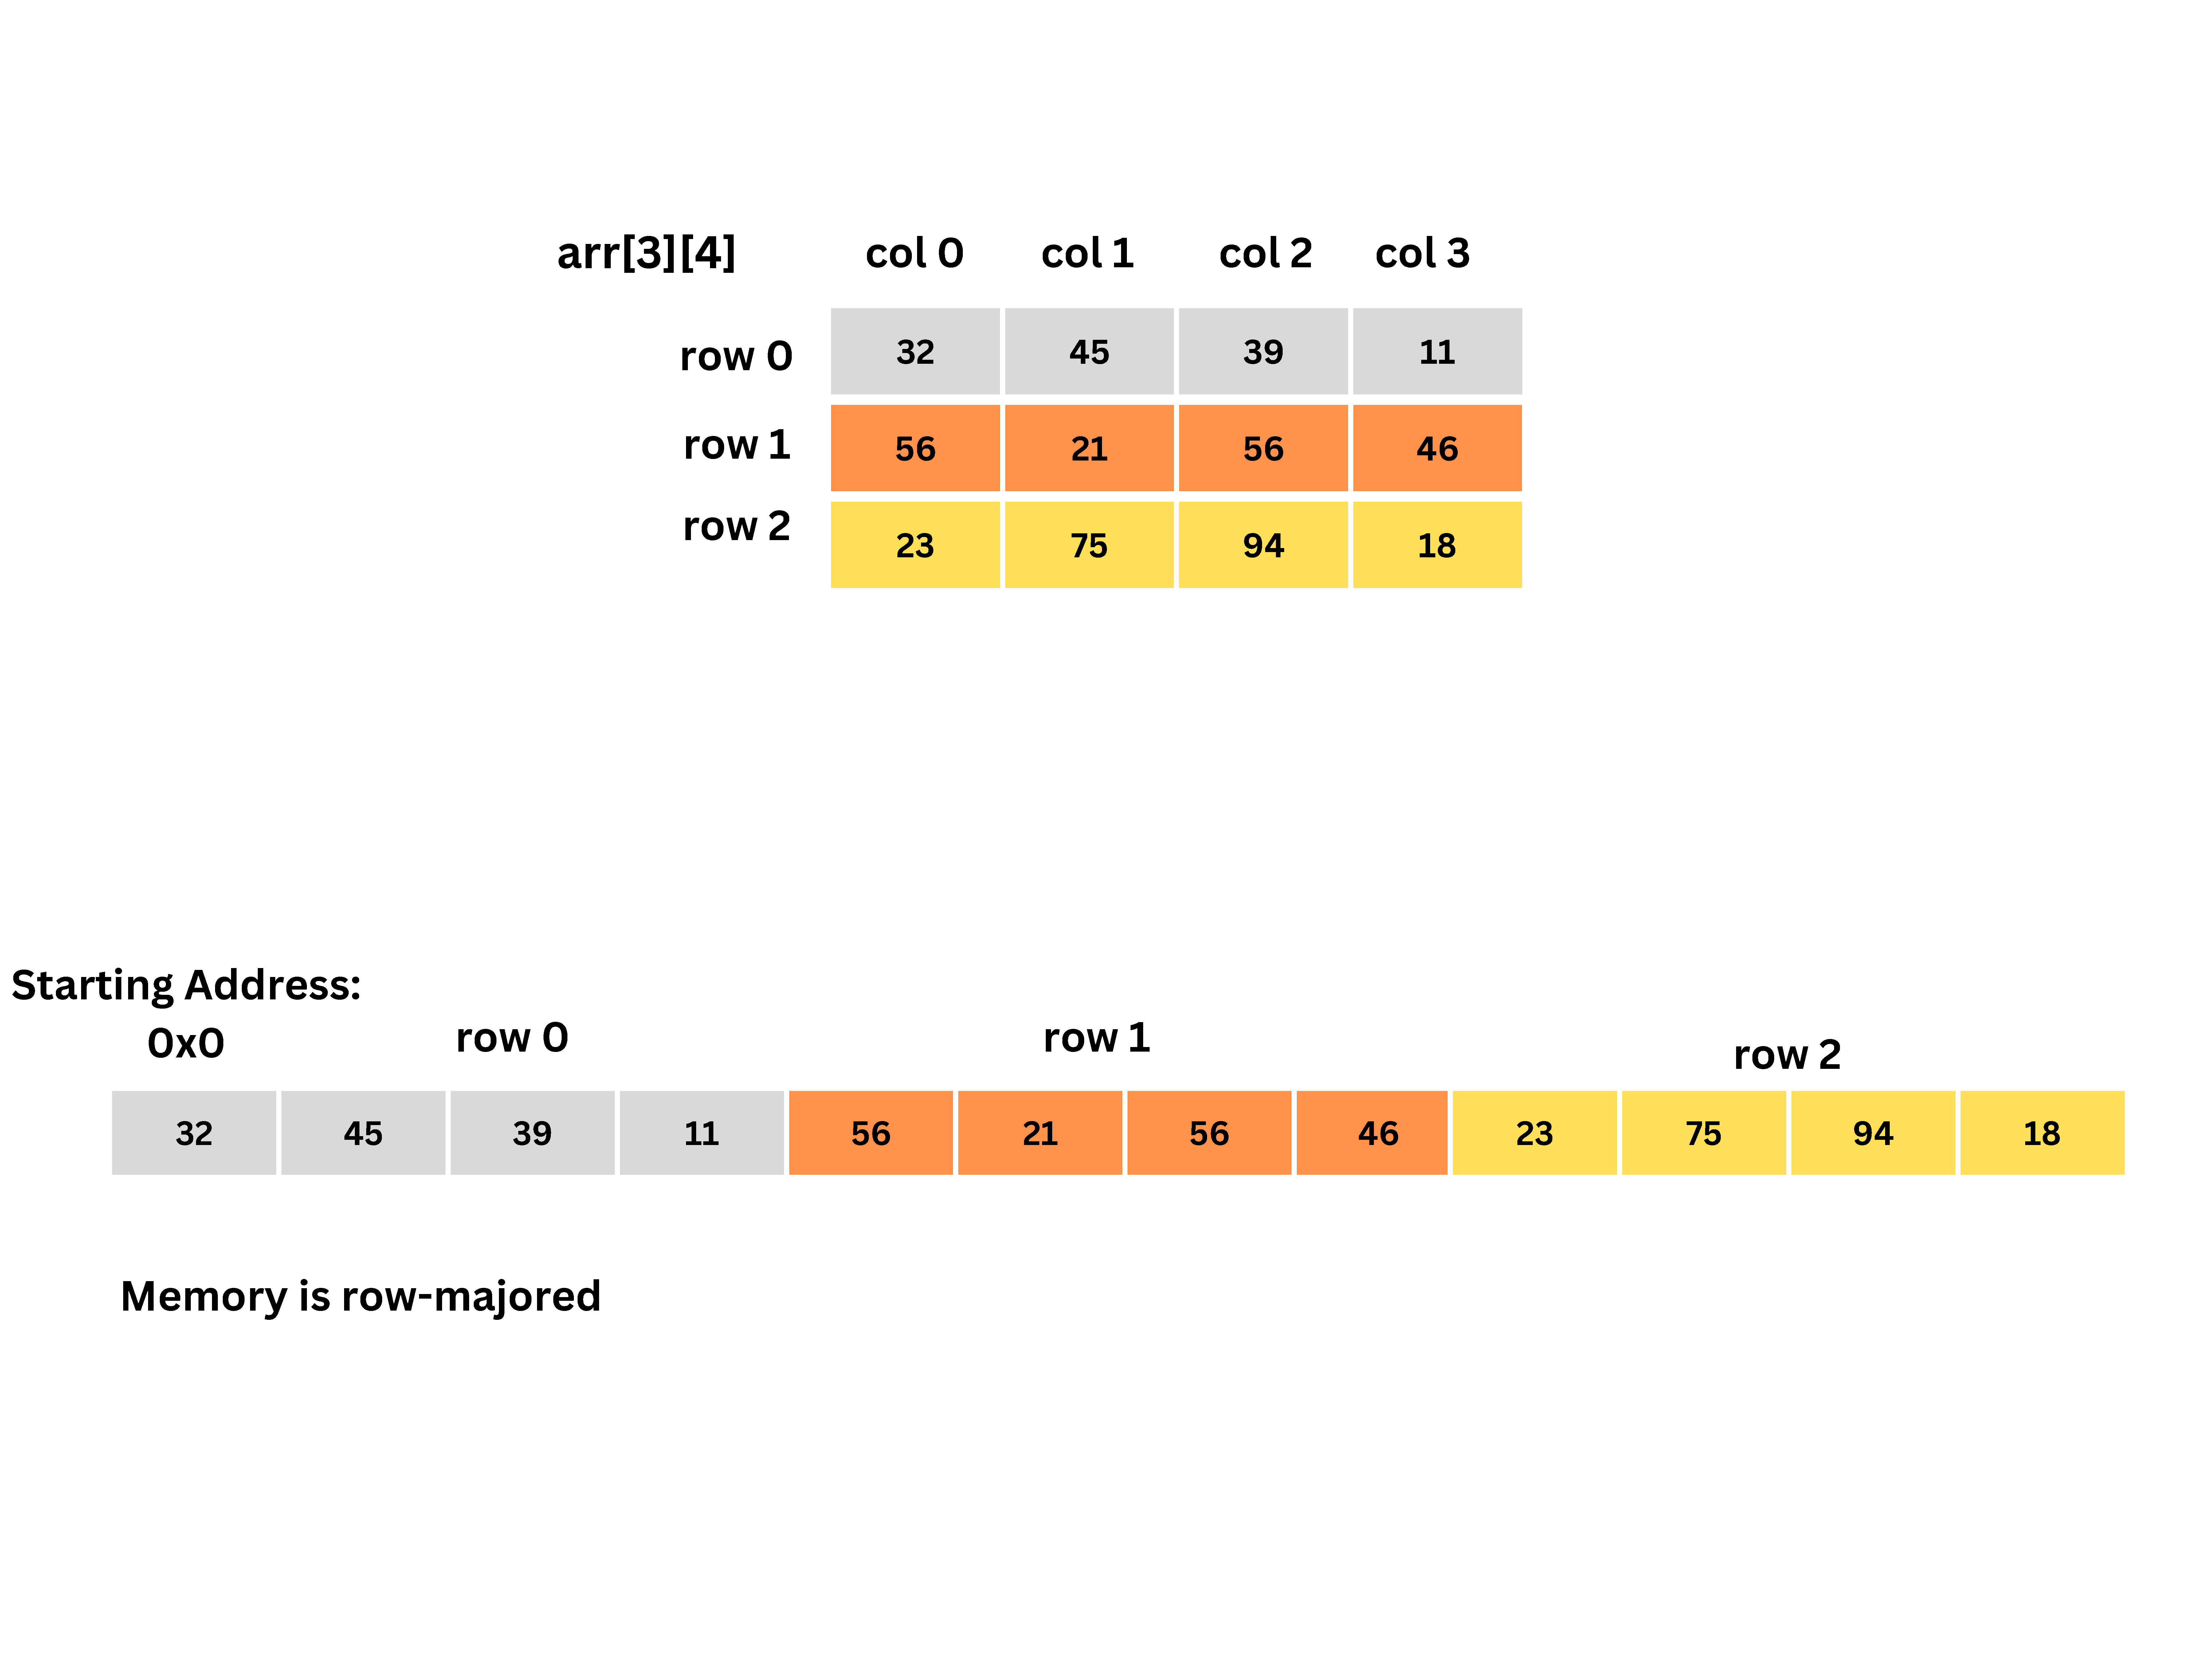
\includegraphics[width=\textwidth]{images/nested_arrays.pdf}
    \caption{Nested Array Diagram. In C arrays are saved in \textit{row-major} order}
    \label{fig:nested_array}
\end{figure}
\\
\noindent Let us consider the array in Figure~\ref{fig:nested_array} as an example: \\
Given the declaration:

\[
\texttt{char arr[3][4];}
\]

where \texttt{char} has \(\text{sizeof}(\texttt{char}) = 1\) byte, the memory address of \(\texttt{arr[1][2]}\) is:

\begin{align*}
arr[2][3] &= arr + \text{sizeof}(\text{Type}) \times (C \times i + j) \\
        &= arr + 1 \times (4 \times 1 + 2) \\
        &= arr + 1 \times (4 + 2) \\
        &= arr + 6
\end{align*}

Thus, \(\texttt{arr[1][2]}\) is located 6 bytes after the base address \( arr \).
Since the array starts at address \texttt{0x0} from the figure, we need the element at address 6 which is 56. \\
\\
\noindent Let us consider another example, \\

Given the declaration:

\[
\texttt{int arr[4][5];}
\]

where \texttt{int} has \(\text{sizeof}(\texttt{int}) = 4\) bytes, we want to find the equivalent \(\texttt{arr[i][j]}\) corresponding to \(\texttt{((int *)arr)[17]}\).

\(\texttt{((int *)arr)[17]}\) means that we cast our 2-D array, to one dimensional integer array. The memory offset of the \texttt{arr[17]} is \texttt{ 17 * sizeof(int)} which is 68. Remember, the equation above is used for the \textbf{memory address} of an element \( A[i][j] \) in a row-major order layout.\\
Now we can apply our equation:

\begin{align*}
arr[i][j] &= arr + \text{sizeof}(int) \times (C \times i + j) \\
        &= arr + 4 \times (5 \times i + j) \\
        &= arr + 20 \times i + 4 \times j
\end{align*}
Since the offset is 68 it means that \[
20 \times i + 4 \times j
\] 
must be equal to \texttt{68} we get \texttt{i = 3} and \texttt{j = 2} using through the following: 

\begin{align*}
20 \times i + 4 \times j &= 68
\end{align*}

Solving for \( i \):

\begin{align*}
i &= \frac{68}{20} = 3 \quad \text{(integer division)}
\end{align*}

Solving for \( j \):

\begin{align*}
j &= 68 \mod 20 = 4 \times j \\
  &=> 8 = 4 \times j \\
  &=> j = 2
\end{align*}

Thus, the equivalent array access form is:
\[
\texttt{arr[3][2]}
\]
\\
You may not need to memorize the equation. Once you understand how nested arrays are stored in \textit{row-major} order, as shown in Figure~\ref{fig:nested_array}, you can easily visualize the memory layout and determine the answer quickly. 

Using the equation is fine as long as you correctly implement \textit{pointer arithmetic} when necessary.

As examples of pointer arithmetic, consider the following declarations:

\begin{verbatim}
char    A[12];
char   *B[8];
int     C[6];
double *D[5];
\end{verbatim}

These declarations will generate arrays with the following parameters:

\begin{table}[h]
    \centering
    \begin{tabular}{c c c c c}
        \toprule
        \textbf{Array} & \textbf{Element size} & \textbf{Total size} & \textbf{Start address} & \textbf{Element i} \\
        \midrule
        A & 1  & 12  & \( x_A \)  & \( x_A + i \) \\
        B & 8  & 64  & \( x_B \)  & \( x_B + 8i \) \\
        C & 4  & 24  & \( x_C \)  & \( x_C + 4i \) \\
        D & 8  & 40  & \( x_D \)  & \( x_D + 8i \) \\
        \bottomrule
    \end{tabular}
\end{table}

\noindent\textbf{Related Problem 17} (Updated from Practice Problem 3.38) \\
Based on the provided assembly code, find the values of \texttt{M} and \texttt{N} for the given C code below:
\begin{verbatim}
long P[M][N];
long Q[N][M];

long sum_element(long i, long j) {
    return P[i][j] + Q[j][i];
}
\end{verbatim}
The assembly code:
\begin{verbatim}
    sum_element:
        leaq    (%rdi,%rdi,2), %rdx
        addq    %rsi, %rdx
        leaq    (%rsi,%rsi,4), %rax
        addq    %rdi, %rax
        movq    Q(,%rax,8), %rax
        addq    P(,%rdx,8), %rax
        ret
\end{verbatim}
\\
\texttt{M} is: \_\_\_ \\
\texttt{N} is: \_\_\_ \\
\\
\textit{Answer: }\url{https://godbolt.org/z/68b4fEc38} \\
\clearpage
\section{Heterogeneous data structures}
\subsection{Struct}
Different ways to declare the structure: \\
\\
\noindent
\begin{minipage}{0.45\textwidth}
\begin{verbatim}
// Standard struct declaration
struct rec {
    int i;
    int j;
    int a[2];
    int *p;
};
\end{verbatim}
\end{minipage}
\hfill
\begin{minipage}{0.45\textwidth}
\begin{verbatim}
// Using typedef with struct
typedef struct rec_t {
    int i;
    int j;
    int a[2];
    int *p;
} rec_t;
\end{verbatim}
\end{minipage}

\vspace{1em}

\noindent
\begin{minipage}{0.45\textwidth}
\begin{verbatim}
// Anonymous struct with typedef
typedef struct {
    int i;
    int j;
    int a[2];
    int *p;
} rec_anonymous;
\end{verbatim}
\end{minipage}

\vspace{1em}

This structure contains four fields: two 4-byte values of type \texttt{int}, a two-element array of type \texttt{int}, and an 8-byte integer pointer, giving a total of 24 bytes:

\begin{table}[h]
    \centering
    \renewcommand{\arraystretch}{1.5}
    \begin{tabular}{c c c c c c}
        \toprule
        \textbf{Offset} & 0 & 4 & 8 & 16 & 24 \\
        \midrule
        \textbf{Contents} & \texttt{i} & \texttt{j} & \texttt{a[0]} & \texttt{a[1]} & \texttt{p} \\
        \bottomrule
    \end{tabular}
\end{table}
\subsection{Padding}
Fields of a \texttt{struct} in C are stored in the order in which they are declared, and the C standard specifies that this order cannot be rearranged in memory. Additionally, many computer systems impose alignment restrictions on \textbf{primitive} data types, requiring that certain objects be placed at addresses that are multiples of a specific value \( K \) (typically 2, 4, or 8). These alignment constraints simplify the design of hardware that interfaces between the processor and the memory system. To satisfy these alignment requirements, padding may be inserted between \texttt{struct} members. \\
\\
\clearpage
The easiest way to determine padding follows two rules:

\begin{enumerate}
    \item Starting from address zero check if the offset where a variable starts is divisible by the size of its type:
    \begin{itemize}
        \item If yes, place it without adding any padding.
        \item If no, round up to the nearest multiple by adding padding.
    \end{itemize}
    
    \item After placing all fields, check the total size of the struct:
    \begin{itemize}
        \item Is the total size divisible by the largest data type's size?
        \item If not, round it up to the nearest multiple by adding padding.
    \end{itemize}
\end{enumerate}
\\
Let us consider the following example:

\noindent\begin{minipage}{0.45\textwidth}
\begin{lstlisting}
typedef struct {
    short a; 
    double b;
    int c;
} my_struct, *p_my_struct;
\end{lstlisting}
\end{minipage}

We have declared \texttt{my\_struct} and \texttt{p\_my\_struct}, which is a pointer to \texttt{my\_struct}. The size of \texttt{p\_my\_struct} is always 8 bytes, as it is a pointer. This is the same as declaring a variable of type \texttt{my\_struct*}. Writing \texttt{p\_my\_struct a;} and \texttt{my\_struct* a;} are equivalent.

Now, let's determine the memory layout of \texttt{my\_struct} using Rule 1.

\begin{enumerate}
    \item \textbf{Starting at address 0:}  
    Is 0 divisible by the size of \texttt{short} (2 bytes)?  
    Yes, because \( 0 \mod 2 = 0 \).  
    We place \texttt{a} at address 0, occupying 2 bytes.

    \item \textbf{Next, adding \texttt{double b}:}  
    The next available address is 2.  
    Is 2 divisible by the size of \texttt{double} (8 bytes)?  
    No, because \( 2 \mod 8 \neq 0 \).  
    To align \texttt{b} properly, we add 6 bytes of padding.  
    Now, \texttt{b} starts at address 8 and occupies 8 bytes.  
    The next available address is \( 8 + 8 = 16 \).

    \item \textbf{Adding \texttt{int c}:}  
    Is 16 divisible by the size of \texttt{int} (4 bytes)?  
    Yes, because \( 16 \mod 4 = 0 \).  
    We place \texttt{c} at address 16, occupying 4 bytes.  
    The total struct size at this point is \( 16 + 4 = 20 \) bytes.

\end{enumerate}

Now, applying Rule 2:

\begin{itemize}
    \item The largest data type in the struct is \texttt{double} (8 bytes).
    \item Is the total struct size (20 bytes) divisible by 8?  
    No, because \( 20 \mod 8 \neq 0 \).
    \item To satisfy alignment requirements, we add 4 bytes of padding at the end to make the total size 24, which is divisible by 8.
\end{itemize}

\textbf{Final Struct Layout:}

\begin{verbatim}
// | a | padding(6) | b       | c  | padding(4) |
// ^0  ^2          ^8        ^16  ^20          ^24
\end{verbatim}

Thus, the final size of \texttt{my\_struct} is \textbf{24 bytes}. \\
See this code and see the output for the same struct: \\

\url{https://godbolt.org/z/anrTEceE1}\\

\\
\\
Please carefully analyze the following examples and understand. They also include nested structs. You can run the examples below here: \url{https://godbolt.org/z/YzohaaoEz} \\
\\
\noindent\begin{minipage}{0.29\textwidth}
\begin{lstlisting}
typedef struct {
    short a; 
    int b;
    int* c;
    short* d;
} p1;  
\end{lstlisting}
\end{minipage}
\begin{minipage}{0.29\textwidth}
\begin{verbatim}
// | a | padding(2) | b | c | d |
//   ^2             ^4  ^8   ^16 
// size = 16 + 8 (short* d) = 24
\end{verbatim}
\end{minipage}

\vspace{1em}

\noindent\begin{minipage}{0.29\textwidth}
\begin{lstlisting}
typedef struct {
    int a[2];
    char b[8];
    short c[4];
    long* d;
} p2;
\end{lstlisting}
\end{minipage}
\begin{minipage}{0.29\textwidth}
\begin{verbatim}
// | a[0] | a[1] | b[0] | b[1] | ... | b[7] | c[0] | ... | c[3] | d
// ^0     ^4     ^8     ^9     ^10          ^16     ^18         ^24
// size = 24 + 8 (long* d) = 32
\end{verbatim}
\end{minipage}

\vspace{1em}

\noindent\begin{minipage}{0.29\textwidth}
\begin{lstlisting}
typedef struct {
    long a[2];
    int* b[2];
} p3;
\end{lstlisting}
\end{minipage}
\begin{minipage}{0.29\textwidth}
\begin{verbatim}
// | a[0] | a[1] | b[0] | b[1]
// ^0     ^8     ^16    ^24
// size = 24 + 8(b[1]) = 32
\end{verbatim}
\end{minipage}

\vspace{1em}

\noindent\begin{minipage}{0.29\textwidth}
\begin{lstlisting}
typedef struct {
    char a[16];
    char* b[2];
} p4, *p_p4;
\end{lstlisting}
\end{minipage}
\begin{minipage}{0.29\textwidth}
\begin{verbatim}
// | a[0] | a[1] | .... | a[15] | b[0] | b[1] 
// ^0     ^1     ^2     ^15     ^16    ^24
// size = 24 + 8(b[1]) = 32
\end{verbatim}
\end{minipage}

\vspace{1em}

\noindent\begin{minipage}{0.29\textwidth}
\begin{lstlisting}
typedef struct {
    p4 a[4];
    p1 b;
} p5;
\end{lstlisting}
\end{minipage}
\begin{minipage}{0.29\textwidth}
\begin{verbatim}
// | a[0] | a[1] | a[2] | a[3] | b
// ^0     ^32    ^64    ^96     ^128 
// size = 128 + 24(b) = 152
\end{verbatim}
\end{minipage}

\vspace{1em}

\noindent\begin{minipage}{0.29\textwidth}
\begin{lstlisting}
typedef struct {
    int a;
    int b;
    long c;
    char d;
    char e;
} p6;
\end{lstlisting}
\end{minipage}
\begin{minipage}{0.29\textwidth}
\begin{verbatim}
// | a | b | c | d | e |
// ^0  ^4  ^8  ^16  ^17
// size = 17 + 7 (!!! The total structure size must be a multiple
// of the largest alignment)
// In our case long is the largest member. 
// Total size must be 24 (rounded up to the nearest multiple of 8).
\end{verbatim}
\end{minipage}
\\
\noindent\textbf{Note:} \\
As you may notice, alignment and our struct padding rules are based on primitive data types. This is why, in the case of \texttt{p5}, we did not apply our rule that checks whether 128 (the size of \texttt{p4 a[4]}) is divisible by 24 (the size of \texttt{p1 b}). Instead, we applied padding based on the alignment requirements of the individual fields.

Additionally, we did not apply our second rule, which checks whether the total size is divisible by the size of the largest field. In this case, the largest field is \texttt{p4}, which has a size of 32 bytes, but the total struct size of 152 is not divisible by 32. Again, this is because we align based on primitive data types.

Since structs do not exist at the assembly level, you can think of nested structs as being "unrolled" into memory, where each nested struct is treated as a contiguous block before aligning the next field.
v

\section{Acknowledgement}. \\
\label{sec:ack}
This document has been created by TA Khagan Karimov for the \textbf{CS-4400 Spring 2025} course as a \textbf{Midterm Review 1} resource. The materials used are based on the textbook \textit{Computer Systems: A Programmer's Perspective (Third Global Edition)} by Randal Bryant and David O'Hallaron, along with lecture slides and notes. Any errors or mistakes are more likely due to my interpretation. If you find an error, please open an issue or submit a pull request here: 
\noindent\url{https://github.com/khagankhan/cs4400-help}

\end{document}
